\section{Dynamic Features}
Physics simulation is the core of DART. The earlier versions of DART
adopted the physics engine, RTQL8 \cite{}, which features forward
simulation based on Lagrangian dynamics
and generalized coordinates. Later, we reimplemented the Featherstone
algorithms using Lie group representation to largely improve the
computation efficiency. The constraint solver, which handles contact,
joint limits, and other Cartesian constraints, has also been optimized
in the later versions of DART. 

\subsection{Lagrangian dynamics and generalized coordinates}
DART is distinguished by its accuracy and stability due to its use of
generalized coordinates to represent articulated rigid body systems,
Featherstone’s algorithm to compute the dynamics of
motion, and Lie group for compact representation and derivation of
dynamic equations.

Articulated human motions can be described by a set of dynamic
equations of motion of multibody systems. Since the direct application
of Newton’s second law becomes difficult when a complex articulated
rigid body system is considered, we use Lagrange’s equations derived
from D'Alembert’s principle to describe the dynamics of motion: 
\begin{equation}
M(\vc{q})\ddot{\vc{q}} + C(\vc{q}, \dot{\vc{q}}) = \vc{Q},
\end{equation}
where $\vc{q}$ is the generalized coordinates that indicate the 
configuration of the skeleton. $M(\vc{q})$ is the mass matrix,
$C(\vc{q},\dot{\vc{q}})$ is the Coriolis and centrifugal term of the
equation of motion, and $\vc{Q}$ is the vector of generalized forces
for all the degrees of freedom in the system.

Once we know how to compute the mass matrix, Coriolis and centrifugal
terms, and generalized forces, we can compute the acceleration in
generalized coordinates, $\ddot{\vc{q}}$ for forward dynamics. Conversely, if we
are given $\ddot{\vc{q}}$ from a motion sequence, we can use these equations of
motion to derive generalized forces for inverse dynamics. However,
directly evaluating the mass matrix and Coriolis term is 
computationally expensive, especially for applications that require
real-time simulation. DART implements Featherstone's articulated rigid
body algorithms to compute forward and inverse dynamics. In addition,
DART uses Lie group representation to further improve efficiency.

\paragraph{Featherstone's algorithms.} In particular, we implement the
recursive Newton-Euler algoritm (RNEA) for inverse dynamics and the
articulated-body algorithm (ABA) for forward dynamics. These two
algorithms are known for their $O(n)$ time with $n$ being the number of
body nodes in the skeleton. 

\paragraph{Lie group representation}
\red{JS} (Describe the high-level ideas of Lie group representation and its advantages).

\subsection{Soft body simulation}
DART is able to simulate soft bodies dynamically coupling with rigid
bodies. For example, one can simulate a robotic gripper with deformable
surface or a humanoid with rubber soles on the feet. The soft body
simulation in DART is based on spring-mass systems described in
generalized coordinates. We use a unified representation for both
rigid and soft bodies so that two-way dynamic coupling can be handled
by the same set of equations of motion (Figure \ref{fig:softbody}. 

\begin{figure*}
\centering
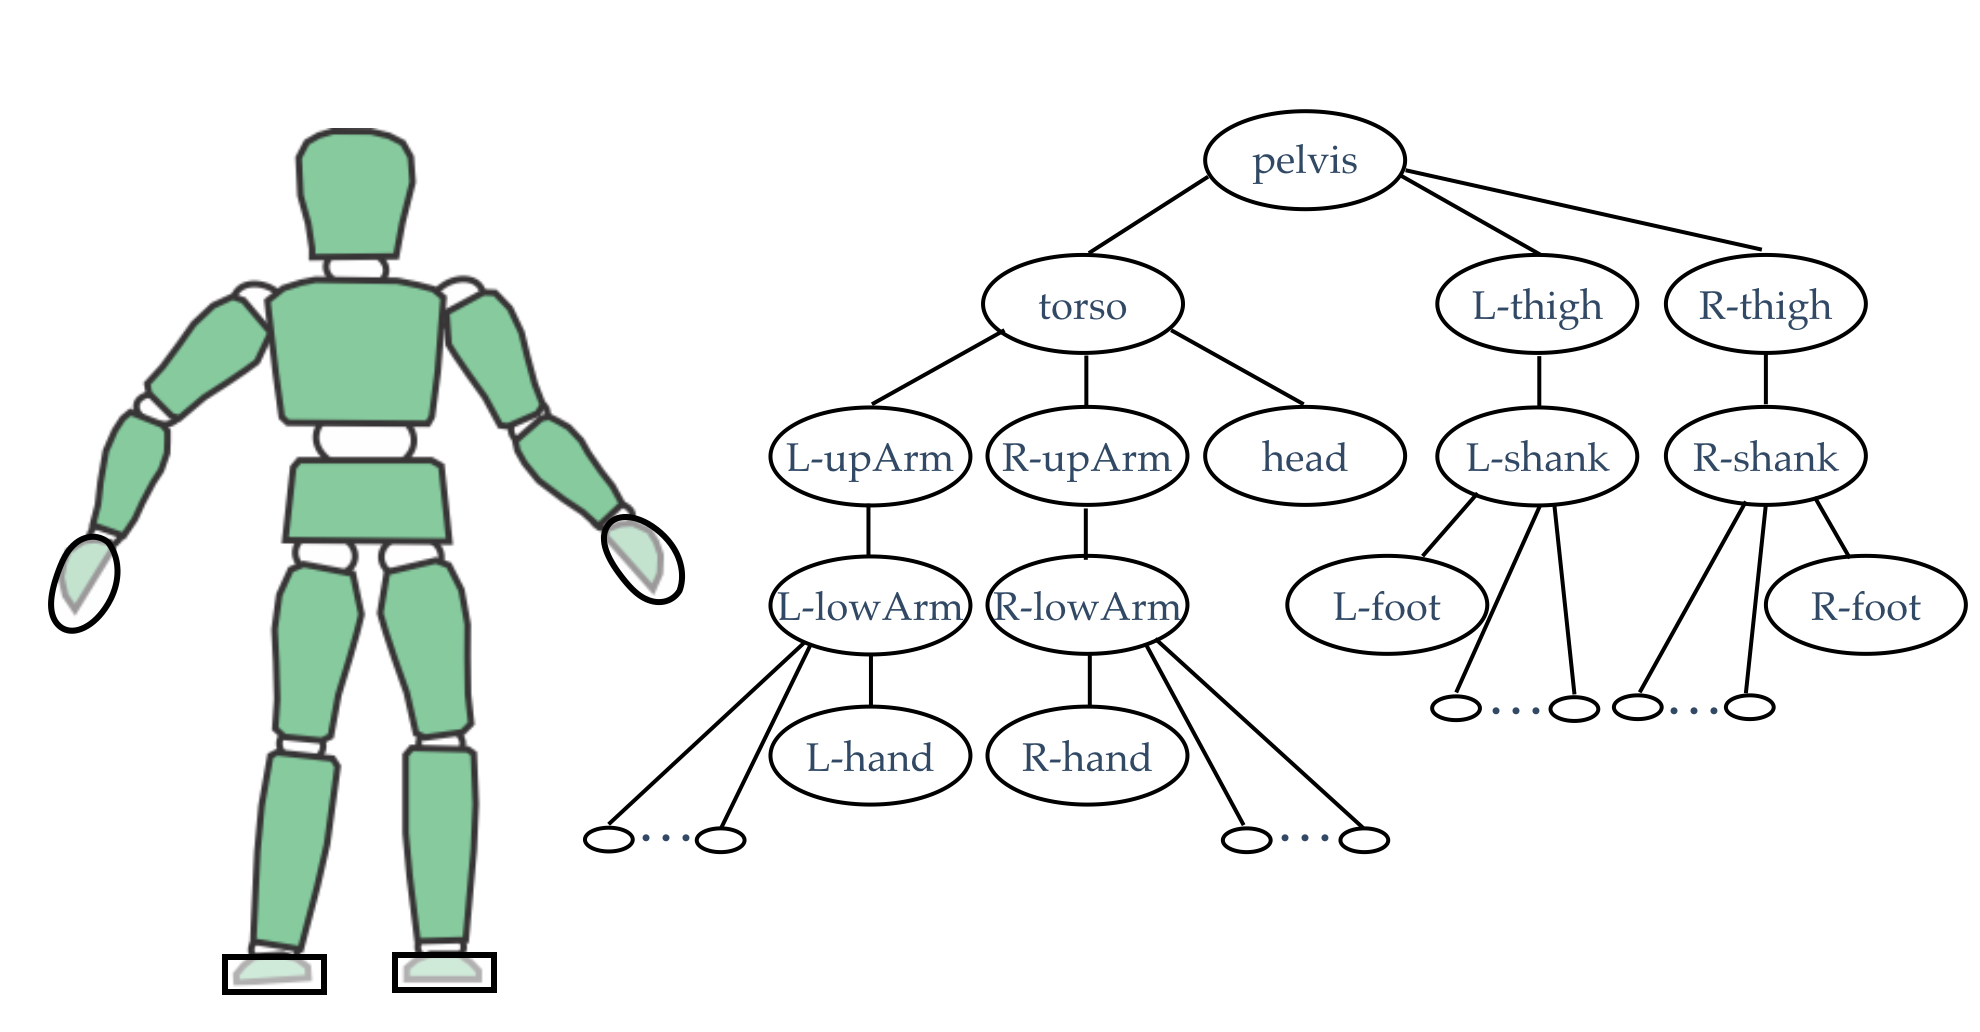
\includegraphics[width=6.0in]{soft-body.jpg}
\caption{The hands and the feet of the humanoid are composed of a
  rigid body with a layer of deformable surface. Both rigid and soft
  bodies are represented in generalized coordinates.}
\label{fig:softbody}
\end{figure*}

Each SoftBodyNode consists of a set of point masses representing the
surface of the deformable part of the body. Each point mass is
attached to the frame of BodyNode as a child link with three translational
degrees of freedom. This compact representation allows us to soften or
harden any part of deformable body at any time, by simply adding or
removing the translational degrees of freedom of involved point
masses, without switching dynamic regimes or introducing any
instability. Based on this flexible representation, we develop an
efficient system where only the site of collision needs to be
simulated as deformable body while the rest of the character remains
rigid.

To make a BodyNode soft, one can simply add a
$<$soft\_shape$>$ element in the $<$body$>$ element in the SKEL file. For
example, if we want to make the left foot of the skeleton
``humanoid'' soft, we will modify the SKEL file as follows:

\begin{lstlisting}[caption=Joint.h]
 <skeleton name="humanoid">
 ...
   <body name="Left foot">
     <gravity>1</gravity>
     <transformation>0 -0.10 0 0 0 0</transformation>
     <inertia>
       <mass>0.5</mass>
       <offset>0 0 0</offset>
     </inertia>
     <soft_shape>
       <total_mass>0.5</total_mass>
       <geometry>
         <box>
           <size>0.5 0.25 0.5</size>
           <frags>3 3 3</frags>
         </box>
       </geometry>
       <kv>500.0</kv>
       <ke>0.0</ke>
       <damp>5.0</damp>
     </soft_shape>
   </body>
...
\end{lstlisting}

The material of the soft body is crucial to the behavior of the soft
body. DART uses four parameters to describe the characteristics of the
soft body:

\begin{enumerate}
\item{Number of point masses ($n$):} The resolution of the soft body surface. 
\item{Shape deformation coefficient ($K_e$):} This parameter
  affects the deformation of the soft body in its material space. 
\item{Surface displacement coefficient ($K_v$)}: This parameter
  affects the displacement of the soft body in the frame of the
  BodyNode. The displacement can be caused by the deformation of the
  shape and the rigid transformation relative to the BodyNode frame.
\item{Damping coefficient ($K_d$):} The damping coefficient of the spring.
\end{enumerate}

\subsection{Joint dynamics}
By default, a joint is completely passive, but DART also provides a
few parameters for the user to model a joint as an angular damped
spring with tunable rest pose, stiffness coefficient, and damping
coefficient.

\begin{lstlisting}[caption=Joint.h]
virtual void setRestPosition(size_t _index, double _q0);
virtual void setSpringStiffness(size_t _index, double _k);
virtual void setDampingCoefficient(size_t _index, double _coeff);
\end{lstlisting}

It is important to note that DART simulates joint dynamics using
implicit integration method which uses the future state to evaluate
the spring and damper forces. The implicit formulation results in
solving a linear system, which is more computational costly, but it
makes the system more stable and allows for larger time step in
simulation.

\subsection{Actuators}
\red{Karen}

\subsection{Constraints}
\red{JS}

\subsection{Accuracy and Performance}
\red{JS}
